% !TEX root = domain_transduction.tex
We evaluate our algorithm on various unsupervised domain adaptation tasks. We perform two sets of experiments one on MNIST and its house-made artificial variant. As well as the standard domain adaptation dataset \emph{Office}\cite{office}. Main motivation behind performing two different sets of experiments is the effect of dataset size; although it is standard,  \emph{Office} dataset is quite small having maximum number of 2478 data points per domain over 31 object classes. We discuss the datasets and their characteristics as well as the baselines in detail in the following sections.

\subsection{Datasets}
In order to evaluate our algorithm, we are using two sets of experiments one on digit classification and the other one on object recognition. 

For digit classification, we are using three different domains as;
\noindent\textbf{MNIST\cite{mnist}:} \emph{MNIST} is a digit classification dataset of 60k images. 
\noindent\textbf{MNIST-M:} As a controlled target domain, we generated a series of digit images by using the original MNIST dataset and the color images of BSDS500\cite{bsds500} following the method explained in \cite{ganin15}. Since the dataset is not distributed directly by the authors, we further confirmed that the performance is similar to experimented in \cite{ganin15}.
\noindent\textbf{SVHN\cite{svhn}:} Street view house numbers dataset is a collection of house numbers collected directly from Google street view images. It is quite interesting because of dataset size as well as the difficulty of the task. There are 600k images in the SVHN\cite{svhn} dataset. Moreover, the adaptation task of MNIST $\rightarrow$ SVHN is proven to be extremely hard and we show the first successful adaptation results for it.

\begin{figure}
\caption{Sample images from MNIST, MNIST-M and SVHN datasets.}
\end{figure}

For object recognition experiment, we are using the \emph{OFFICE}\cite{office} dataset and it has three domains as
\noindent\textbf{Amazon:} Images of objects with white background directly taken from Amazon.
\noindent\textbf{Webcam:} Images of the same objects taken with a webcam on a complicated background.
\noindent\textbf{D-SLR:} Images of the same objects taken with a high resultion D-SLR.

\begin{figure}
\caption{Sample images from Amazon, Webcam and D-SLR domains of the Office dataset.}
\end{figure}


\subsection{Baselines}
\subsection{Implementation Details}
\subsubsection{Feature Extraction - CNN Architectures}
In all of our experiments, we are using 128 dimensional features extracted using convolutional neural networks. For each experiment, we are using a different architecture mostly because of the dataset size.

For digit classification experiments, we are using 5-layer networks of;
\begin{figure}[h]
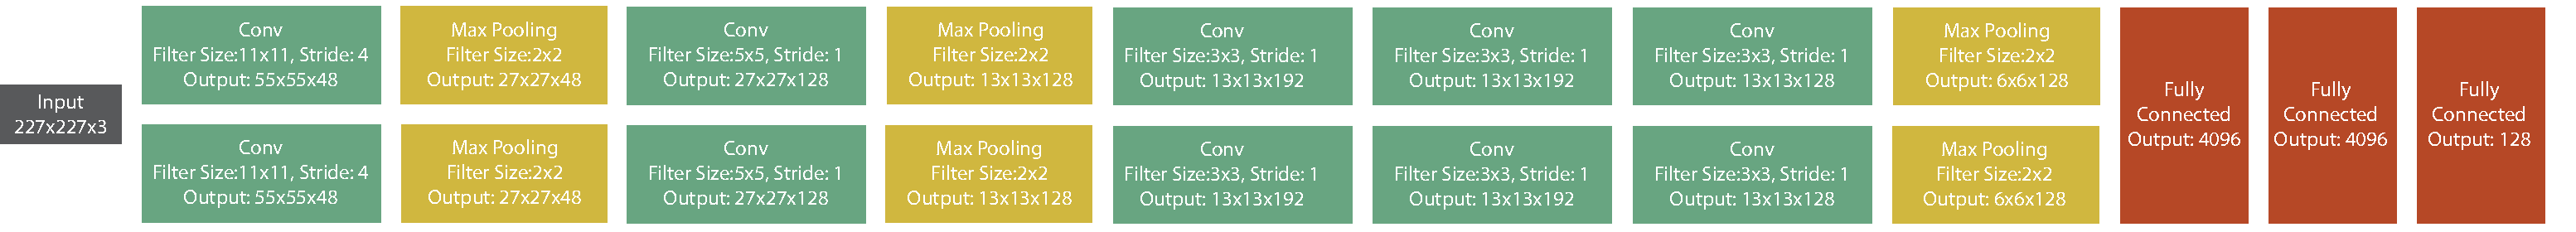
\includegraphics[width=\columnwidth]{alexnet}
\caption{Feature Extraction Network - Modified AlexNet}
\end{figure}
We learn all parameters directly from the data using AdaGrad\cite{adagrad} and initialize with truncated normals having unit variance. We use the learning rate $2.5x10^{-3}$ and the batch size $256$.

Moreover; for object recognition experiment, we are using the AlexNet architecture\cite{alexnet};
\begin{figure}[h]
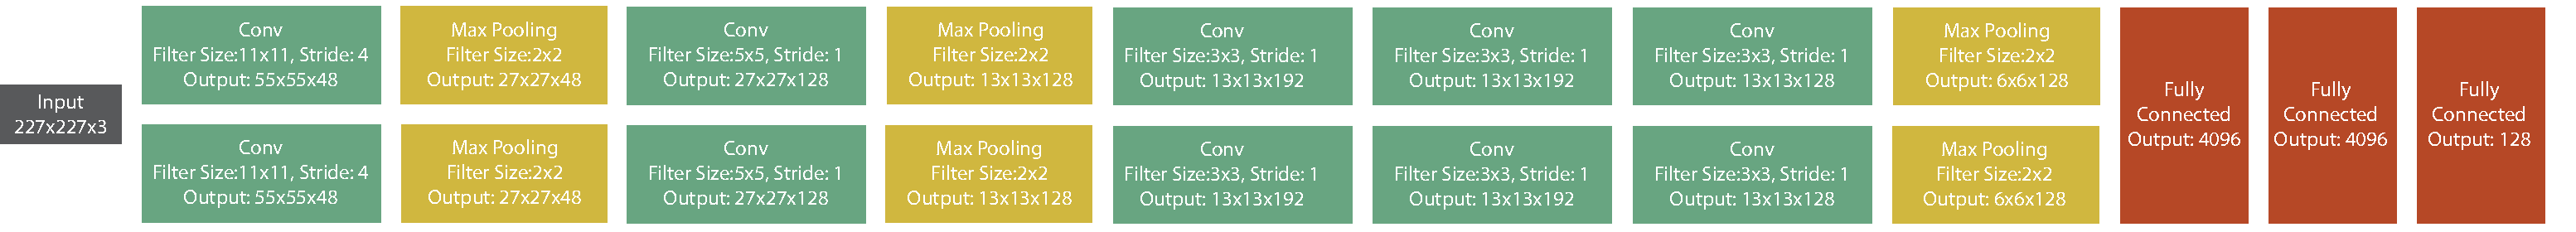
\includegraphics[width=\columnwidth]{alexnet}
\caption{Feature Extraction Network - Modified AlexNet}
\end{figure}
Due to the scarcity of the data, we use the parameters pre-trained on ImageNet for all layers except  last fully connected layer. We further extend the network with fully connected layer of dimensionality reduction to 128D. We learn the fc-7 and fc-8 using AdaGrad\cite{adagrad} and initialize with truncated normals having unit variance. We use the learning rate $2.5x10^{-4}$ and the batch size $256$. 

We further share our learned models as well as the source code using TensorFlow\cite{tensorflow} on \url{anonymous.xyz}

\subsection{Evaluation Procedure}
We are evaluating all of the algorithms using the \emph{fully-transductive} setting. In other words,  we feed training set of source and target to our transductive domain adaptation algorithm. As an evaluation, we directly evaluate the labels obtain for the target unsupervised training data. We report the accuracy as the learning metric. Accuracy is the ratio of the correctly classified data points to the target unsupervised training data points.

\subsection{Results}
\subsubsection{Effect of label propogation and feature laerning}
In order to evaluate the effect of having a robust label propagation and feature learning, we compare our method with a variant without the label propagation (noted as \emph{our-method-no-prop}) and a variant without feature learning (noted as \emph{our-method-no-fl}). We plot the accuracy vs number of iterations in order to evaluate both the effect on learning rate as well as the resultant accuracy. Although we plot the results only for MNIST$\rightarrow$MNIST-M, the other experiments have similar results and not displayed for the sake of clarity. Results are show in the Figure~\ref{fllprop}. 
  
\begin{figure}[ht]
\caption{Accuracy vs number of iterations for our-method, our-method-no-prop and our-method-no-fl. As the figure suggests the label propagation both increase the learning rate as well as the final accuracy. Moreover, the feature learning also have a significant effect on the accuracy.}
\label{fllprop}
\end{figure}
\begin{table*}[t]
\resizebox{\textwidth}{!}{
\begin{tabular}{@{}rcccccccc@{}} \toprule 
 Source & Amazon & D-SLR & Webcam & Webcam &Amazon & D-SLR & MNIST-M & MNIST \\
 Target & Webcam & Webcam & D-SLR & Amazon & D-SLR & Amazon & MNIST & MNIST-M\\
 \midrule
GFK \cite{gong2012} & $.398$ & $.791$ & $.746 $ & $.371$ & $.379$ & .379 &  &  \\
SA* \cite{fernando13} & $.450$ & $.648$ & $.699$ & $.393$ & $.388$ & $.420$ &  & $.567$\\
DLID \cite{chopra13} & $.519$ & $.782$ & $.899$ & & & & &\\
DDC \cite{tzeng14} & $.618$ & $.950$ & $.985$ & $.522$ & $.644$& $.521$& &\\
DAN \cite{wang15} & $.685$ & $.960$ & $.990$ & $.531$ & $.670$ & $.540$ & $$ &\\
Backprop \cite{ganin15} & $.730$ &$\mathbf{.964}$ & $\mathbf{.992}$ & & & & & $.771$ \\
\midrule
Source Only & $.642$ & $.961$ & $.978$ & & & & & $.524$ \\
Our Method & $\mathbf{.781}$ &.930 & $.987$ & $.625$ & $.839$ & $.567$ & $.835$ & $\mathbf{.855}$\\
 \bottomrule
\end{tabular}}
\end{table*}